% ----------------------------------------------------------
\begin{frame}
  \frametitle{Problem-Specific Qubit Scaling}
  Problem: Factor 2048-bit number

  Solution: Design device for Shor's algorithm with logical qubits, ancilla
  generation, connections, surface code error correction, and imperfect
  device yield~\cite{acm-qcomp-blueprint}
    
  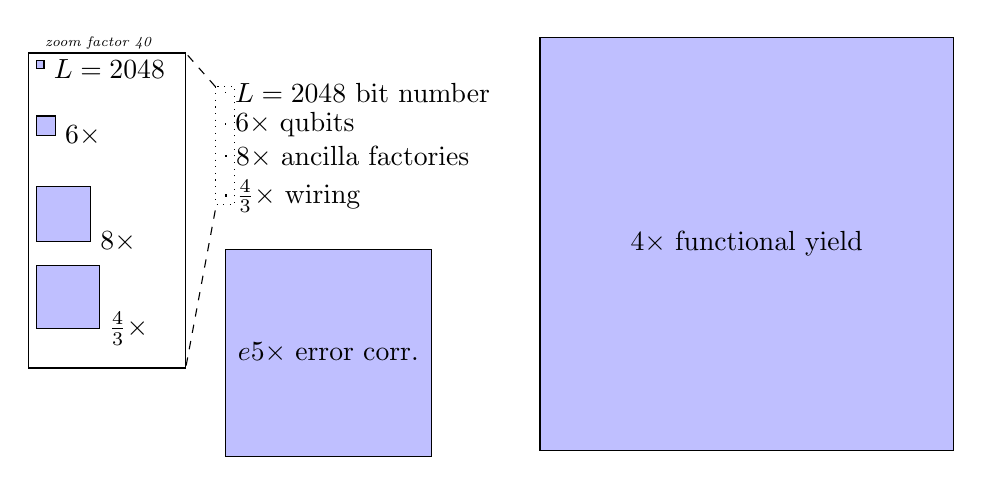
\begin{tikzpicture}[x=1mm, y=1mm, qubits/.style={fill = blue!25}]
    \def\baseLen{0.025}
    \def\shiftLen{1}
    \draw [qubits] (0,0) rectangle %
    +(\baseLen, -\baseLen) %
    node [right] {$L=2048$ bit number}; %
    
    \draw [qubits] (0,-4*\shiftLen) rectangle %
    +(sqrt 6*\baseLen, -sqrt 6*\baseLen) %
    node [right] {$6\times$ qubits}; %
    
    \draw [qubits] (0,-8*\shiftLen) rectangle %
    +(sqrt 48*\baseLen, -sqrt 48*\baseLen) %
    node [right] {$8\times$ ancilla factories}; %
    
    \draw [qubits] (0,-13*\shiftLen) rectangle %
    +(sqrt 64*\baseLen, -sqrt 64*\baseLen) %
    node [right] {$\frac{4}{3}\times$ wiring}; %
    
    \draw [qubits] (0,-20*\shiftLen) rectangle %
    +(1049*\baseLen, -1049*\baseLen) %
    node [midway] {$\num{e5}\times$ error corr.};
    
    \draw [qubits] (40*\shiftLen,7*\shiftLen) rectangle %
    +(2100*\baseLen, -2100*\baseLen) %
    node [midway] {$4\times$ functional yield}; %

    \coordinate (ULsmall) at (-50*\baseLen, 30*\baseLen);
    \coordinate (LLsmall) at (-50*\baseLen, -15*\shiftLen);
    \draw [dotted] (ULsmall) rectangle +(100*\baseLen, -15*\shiftLen);

    % Increase base length 
    \def\baseLen{1}
    % Make the zoom box
    \draw (-25*\baseLen, 5*\baseLen) rectangle +(20*\baseLen,
    -40*\shiftLen);
    \draw [dashed] (ULsmall) -- (-5*\baseLen, 5*\baseLen);
    \draw [dashed] (LLsmall) -- (-5*\baseLen, -35*\baseLen);
    \node [label=above:\emph{\tiny{zoom factor 40}}] (zoomBox) at (-16*\baseLen, 3*\shiftLen) {};
    \draw [qubits] (-24*\baseLen, 4*\shiftLen) rectangle %
    +(\baseLen, -\baseLen) %
    node [right] {$L=2048$}; %
    
    \draw [qubits] (-24*\baseLen,-3*\shiftLen) rectangle %
    +(sqrt 6*\baseLen, -sqrt 6*\baseLen) %
    node [right] {$6\times$}; %
    
    \draw [qubits] (-24*\baseLen,-12*\shiftLen) rectangle %
    +(sqrt 48*\baseLen, -sqrt 48*\baseLen) %
    node [right] {$8\times$}; %
    
    \draw [qubits] (-24*\baseLen,-22*\shiftLen) rectangle %
    +(sqrt 64*\baseLen, -sqrt 64*\baseLen) %
    node [right] {$\frac{4}{3}\times$}; %
  \end{tikzpicture}
\end{frame}
